\documentclass{article}
\usepackage{iclr2026_conference,times}
\input{math_commands.tex}

\usepackage{hyperref}
\usepackage{url}
\usepackage{amsmath,amssymb,amsthm}
\usepackage{booktabs}
\usepackage{tikz}
\usetikzlibrary{arrows.meta,positioning,calc}

\definecolor{accent}{RGB}{196,58,90}

\newtheorem{proposition}{Proposition}
\newtheorem{theorem}{Theorem}
\theoremstyle{definition}
\newtheorem{definition}{Definition}

% \Cov and \Var come from math_commands.tex
\DeclareMathOperator{\Exp}{\mathbb{E}}
\newcommand{\Cobs}{C_{\mathrm{obs}}}
\newcommand{\Ccert}{C_{\mathrm{cert}}}
\newcommand{\Dcert}{D_{\mathrm{cert}}}

\title{What Survives a Frozen Generative Channel,\\ and to Whom}

\author{Anonymous}

\newcommand{\fix}{\marginpar{FIX}}
\newcommand{\new}{\marginpar{NEW}}

\iclrfinalcopy

\begin{document}
\maketitle

\begin{abstract}
\textbf{[Abstract written last: its final claim depends on the Phase A outcome.]}
A frozen text-to-image diffusion model is a channel from its initial latent $Z$ to the
image it produces. We ask what information about $Z$ remains recoverable from the image
after transmission, and show that the right object is not a scalar capacity but a
\emph{geometry}: the covariance of the Bayes posterior mean,
$\Cobs=\Cov(\Exp[Z\mid Y])$, whose eigenvectors are latent directions ordered by how much
of their prior uncertainty an observer can remove. Because the Bayes decoder is
unavailable, we give an estimator that is a \emph{certificate} rather than a proxy: for
any decoder $f$, $\Ccert(f)=\Cobs-\Cov(m-f)\preceq\Cobs$, so every direction it reports
is one the channel really carries. We then observe that observability is not a property
of the channel alone. Writing $\Cobs(\mathcal I_R)$ for a receiver with information set
$\mathcal I_R$, the tower property gives
$\Cobs(Y,S)\succeq\Cobs(Y)$ for any side information $S$: knowing what the generator was
conditioned on can only enlarge the observable geometry, never shrink it. We instantiate
this on Stable Diffusion v1.5 with a four-arm capacity- and distribution-matched ladder
that isolates \emph{paired} conditioning from architecture and from the conditioning
marginal.
\end{abstract}

\section{Introduction}

A generative model that is used the same way twice is a channel. Fix the weights, fix the
sampler, and the map from an initial latent $Z$ to the produced image $X=G(Z,S)$ is a
deterministic function; put the image through compression, resizing or noise and the
observation $Y$ is a channel output. This view is implicit whenever anyone hides
information in generated content, edits an image by moving its latent, or asks whether a
sample can be traced back to its seed. It is rarely made explicit, and when it is, it is
usually reduced to a single number: how many bits survive.

\paragraph{The dominant view, stated fairly.}
Work on latent-space watermarking and inversion asks \emph{which} encoding to use --- which
subspace, which pattern, which decoder --- and reports one aggregate: bit error rate under
a set of attacks. That is a reasonable engineering target, and for a deployed watermark it
is the target. It also quietly assumes that the channel treats the latent isotropically,
so that the encoding is a design choice made against a featureless background.

\paragraph{What that framing hides.}
However, this perspective obscures a prior question: \emph{is the background featureless?}
A frozen generative channel does not attenuate every latent direction equally. Some
directions of $Z$ leave a strong, recoverable imprint on the image; others are consumed by
the sampler and the decoder and leave essentially nothing. An aggregate bit rate averages
over that structure and therefore cannot distinguish ``this encoding is bad'' from ``this
direction was never observable.'' Worse, it cannot distinguish either from a third
possibility that turns out to matter: ``this direction is not observable \emph{to this
receiver}.''

\paragraph{The object we propose.}
We replace the scalar with a geometry. For a receiver that sees $Y$, define
\[
  \Cobs \;=\; \Cov\bigl(\Exp[Z\mid Y]\bigr),
\]
the covariance of the Bayes posterior mean. Its quadratic form has a direct reading:
$v^\top\Cobs v=\Var(\Exp[v^\top Z\mid Y])$, and when $Z\sim\mathcal N(0,I)$ this equals
$1-\Exp[\Var(v^\top Z\mid Y)]$ --- the fraction of direction $v$'s prior uncertainty an
observer can remove. Its eigendecomposition $\Cobs=V\Lambda V^\top$ orders latent
directions by observability, and the leading eigenspace is the most observable latent
subspace. A scalar capacity is a trace; the geometry is the object the trace summarises.

\paragraph{Making it estimable without the Bayes decoder.}
$\Exp[Z\mid Y]$ is not available. The tempting substitute, $\Cov(f(Y))$ for a trained
decoder $f$, is not a bound in either direction: a badly scaled decoder can report more
apparent observability than the channel contains. We instead use
\[
  \Ccert(f)\;=\;\Exp\bigl[z_c f_c^\top + f_c z_c^\top - f_c f_c^\top\bigr]
  \;=\;\Cobs-\Cov(m-f)\;\preceq\;\Cobs ,
\]
which is a \emph{certificate}: whatever it reports, the channel carries at least that much.
The price is that $\Ccert$ is indefinite, and that is not a technicality --- it is what
distinguishes a certificate from a proxy, and it changes how the object must be estimated
and drawn.

\paragraph{Observable to whom.}
The final step is that $\Cobs$ is not a property of the channel alone. Write
$\Cobs(\mathcal I_R)=\Cov(\Exp[Z\mid\mathcal I_R])$ for a receiver with information set
$\mathcal I_R$. A blind receiver has $\mathcal I_b=Y$; a receiver that also knows the
conditioning the generator used has $\mathcal I_s=(Y,S)$. Since
$\Exp[\Exp[Z\mid Y,S]\mid Y]=\Exp[Z\mid Y]$, the law of total covariance gives
$\Cobs(Y,S)-\Cobs(Y)=\Exp[\Cov(\Exp[Z\mid Y,S]\mid Y)]\succeq0$. Side information cannot
reduce observability, and may enlarge it \emph{directionally}. Whether it does so
materially for a real diffusion channel is an empirical question, and it is the one our
main experiment is designed to answer.

\paragraph{Contributions.}
\begin{itemize}
  \item \textbf{Framework.} Latent observability through a frozen generative channel as a
  geometry $\Cobs$ rather than a scalar rate, with a linear--Gaussian bridge showing it is
  the global Bayesian counterpart of the local Fisher geometry.
  \item \textbf{Estimator.} A decoder-certified operator $\Ccert(f)\preceq\Cobs$ with a
  cross-fitted, held-out, bootstrap-bounded estimator, and the reasons $\Cov(f)$ and
  diagonal clipping fail.
  \item \textbf{Receiver conditioning.} Monotonicity of observability in the receiver's
  information set, together with an explicit statement of why the difference of two
  certificates does \emph{not} inherit it.
  \item \textbf{Experiments.} \textbf{[Phase A pending.]}
\end{itemize}

\section{Method}

\subsection{Bayesian observability geometry of frozen generative channels}
\label{sec:geometry}

\emph{What is observable?}

Let $Z\sim\mathcal N(0,I_d)$ be the initial latent, $S$ the conditioning actually supplied
to the generator, $X=G(Z,S)$ the produced image with $G$ frozen, and $Y=T(X)$ the
observation after a transmission channel $T$ (compression, resizing, noise, blur). The
receiver sees $Y$ and nothing else unless stated otherwise.

\begin{definition}[Observability operator]
$\Cobs=\Cov\bigl(\Exp[Z\mid Y]\bigr)$.
\end{definition}

Its quadratic form is the quantity of interest:
$v^\top\Cobs v=\Var\bigl(\Exp[v^\top Z\mid Y]\bigr)$, and by the law of total variance,
for $\|v\|=1$ and $Z\sim\mathcal N(0,I)$,
\begin{equation}
  v^\top\Cobs v \;=\; 1-\Exp\bigl[\Var(v^\top Z\mid Y)\bigr] \;\in\;[0,1].
  \label{eq:quadform}
\end{equation}
So $v^\top\Cobs v$ is the fraction of the prior uncertainty in direction $v$ that an
observation removes: $1$ means $v^\top Z$ is recoverable, $0$ means the channel destroyed
it. Writing $\Cobs=V\Lambda V^\top$, eigenvectors are observable latent directions,
eigenvalues are direction-wise observability strengths, and the top-$k$ eigenspace is the
most observable $k$-dimensional latent subspace. Figure~\ref{fig:geometry} is this
definition and nothing else.

\begin{figure}[t]
\centering
% Fig. 2 -- what "observable" means. One inference: an isotropic prior becomes an
% anisotropic observability ellipsoid, direction by direction.
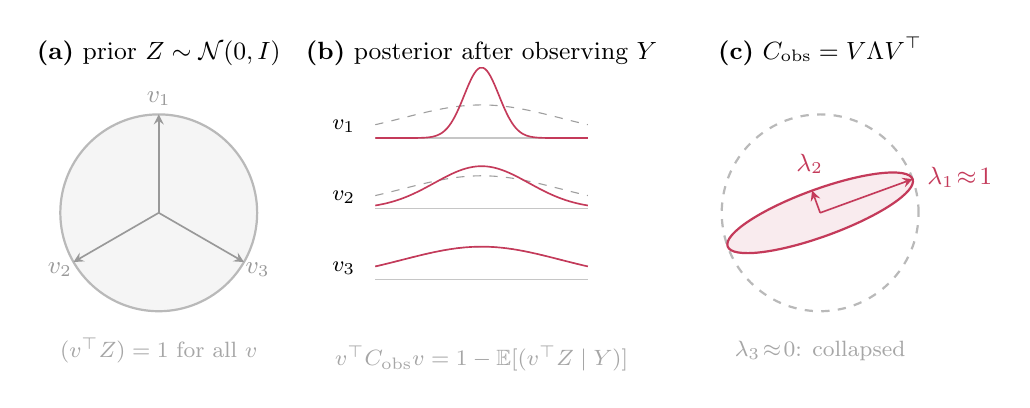
\begin{tikzpicture}[scale=1.0,
  every node/.style={font=\small},
  ax/.style={->,>=stealth,thin,gray!70},
  dir/.style={->,>=stealth,semithick},
  prior/.style={draw=gray!55,fill=gray!8,thick},
  post/.style={draw=accent,fill=accent!10,thick}]

% ---------- (a) isotropic prior ----------
\begin{scope}[shift={(0,0)}]
  \node[anchor=south] at (0,1.75) {\textbf{(a)} prior $Z\sim\mathcal N(0,I)$};
  \draw[prior] (0,0) circle (1.25);
  \foreach \a/\l in {90/{$v_1$},210/{$v_2$},330/{$v_3$}}
    \draw[dir,gray!80] (0,0) -- (\a:1.25) node[pos=1.16] {\l};
  \node[font=\footnotesize,gray!70] at (0,-1.75) {$\Var(v^\top Z)=1$ for all $v$};
\end{scope}

% ---------- (b) posterior narrowing, direction by direction ----------
\begin{scope}[shift={(4.1,0)}]
  \node[anchor=south] at (0,1.75) {\textbf{(b)} posterior after observing $Y$};
  \foreach \i/\y/\s/\lab in {1/0.95/0.22/{$v_1$},2/0.05/0.60/{$v_2$},3/-0.85/1.00/{$v_3$}}{
    \draw[gray!45] (-1.35,\y) -- (1.35,\y);
    \draw[domain=-1.35:1.35,samples=60,smooth,gray!75,thin,dashed]
      plot (\x,{\y+0.42*exp(-(\x*\x)/(2*1.0*1.0))});
    \draw[domain=-1.35:1.35,samples=60,smooth,accent,semithick]
      plot (\x,{\y+0.42*(1.0/\s)^0.5*exp(-(\x*\x)/(2*\s*\s))});
    \node[font=\footnotesize] at (-1.75,\y+0.15) {\lab};
  }
  \node[font=\footnotesize,gray!70,align=center] at (0,-1.85)
    {$v^\top C_{\mathrm{obs}} v = 1-\Exp[\Var(v^\top Z\mid Y)]$};
\end{scope}

% ---------- (c) the ellipsoid ----------
\begin{scope}[shift={(8.4,0)}]
  \node[anchor=south] at (0,1.75) {\textbf{(c)} $C_{\mathrm{obs}}=V\Lambda V^\top$};
  \draw[prior,dashed,fill=none] (0,0) circle (1.25);
  \draw[post,rotate=20] (0,0) ellipse (1.25 and 0.30);
  \draw[dir,accent,rotate=20] (0,0) -- (1.25,0) node[right,pos=1.05] {$\lambda_1\!\approx\!1$};
  \draw[dir,accent,rotate=20] (0,0) -- (0,0.30) node[above,pos=1.3] {$\lambda_2$};
  \node[font=\footnotesize,gray!70] at (0,-1.75) {$\lambda_3\!\approx\!0$: collapsed};
\end{scope}
\end{tikzpicture}

\caption{Observability is anisotropic even when the prior is not. (a) Every unit direction
starts with the same prior variance. (b) Observing $Y$ narrows the posterior by different
amounts in different directions; dashed grey is the prior, solid colour the posterior.
(c) Collecting those numbers gives $\Cobs$, an ellipsoid inside the prior ball whose axes
are the observable directions and whose lengths are $\lambda_j=1-\Exp[\Var(v_j^\top Z\mid
Y)]$. A scalar bit rate is the trace of this object.}
\label{fig:geometry}
\end{figure}

\paragraph{Relation to Fisher information.}
The definition is global and Bayesian; the familiar local object is not. The two agree in
the linear--Gaussian case, which locates $\Cobs$ rather than replacing it.

\begin{proposition}[Fisher bridge]
\label{prop:fisher}
Let $Y=AZ+\varepsilon$ with $Z\sim\mathcal N(0,I)$, $\varepsilon\sim\mathcal N(0,\Sigma_
\varepsilon)$ independent, and let $J_F=A^\top\Sigma_\varepsilon^{-1}A$ be the Fisher
information of $Y$ about $Z$. Then
\[
  \Cobs \;=\; J_F\,(I+J_F)^{-1},
\]
so $\Cobs$ and $J_F$ share eigenvectors and $\lambda_{\mathrm{obs},j}=\lambda_{F,j}/(1+
\lambda_{F,j})$.
\end{proposition}
\begin{proof}
The posterior precision is $I+J_F$, so $\Cov(Z\mid Y)=(I+J_F)^{-1}$ and
$\Cobs=\Cov(Z)-\Exp[\Cov(Z\mid Y)]=I-(I+J_F)^{-1}=J_F(I+J_F)^{-1}$.
\end{proof}

Fisher information asks whether two nearby latent states are locally distinguishable;
$\Cobs$ asks how much of a direction is globally inferable under the prior. The map
$\mu\mapsto\mu/(1+\mu)$ compresses an unbounded local quantity into $[0,1)$, which is
exactly the range that \eqref{eq:quadform} predicts and that our implementation
enforces as an invariant on every estimated spectrum.

\subsection{Decoder-certified observability}
\label{sec:certificate}

\emph{How can observability be measured without knowing the Bayes decoder?}

$m(Y)=\Exp[Z\mid Y]$ is unavailable, so let $f$ be a decoder trained to approximate it.
The natural substitute $\Cov(f(Y))$ is not usable: it is not a lower bound on $\Cobs$ for
an approximate decoder, and its error grows with the decoder's scale rather than with its
quality. We use instead, with $z_c,f_c$ the centred latent and decoder output,
\begin{equation}
  \Ccert(f)\;=\;\Exp\bigl[z_cf_c^\top+f_cz_c^\top-f_cf_c^\top\bigr].
  \label{eq:ccert}
\end{equation}

\begin{theorem}[Certificate]
\label{thm:cert}
For any square-integrable $f$, $\ \Ccert(f)=\Cobs-\Cov(m-f)\preceq\Cobs$, with equality
iff $f=m$ almost surely.
\end{theorem}

\noindent\textbf{Consequence.} Every direction $\Ccert$ reports is one the channel really
carries: a better decoder can only raise the certificate, never inflate it past the truth.
This is what makes the estimate falsifiable rather than merely optimistic.

\paragraph{$\Ccert$ is indefinite, and that is the point.}
$\Cov(f)$ is positive semidefinite by construction --- which is precisely why it cannot be
a bound. $\Ccert$ can have negative eigenvalues, and their magnitude measures decoder
misspecification in that direction. Two consequences follow and both are easy to get
wrong. First, any solver that ranks by $|\lambda|$ --- every SVD-based routine --- returns
the directions the decoder is \emph{worst} on as the leading ones; the eigensolver must be
algebraically largest. Second, $\Ccert\preceq\Cobs$ orders quadratic forms, not volumes:
drawing the certificate as a smaller ellipsoid nested inside $\Cobs$ is wrong whenever
$\Ccert$ has a negative direction. Figure~\ref{fig:certificate} draws it as a signed
spectrum instead.

\begin{figure}[t]
\centering
% Fig. 3 -- why the certificate is NOT a smaller ellipsoid inside a bigger one.
% One inference: C_cert is indefinite, so the object we can estimate has negative
% directions that Cov(f) can never express.
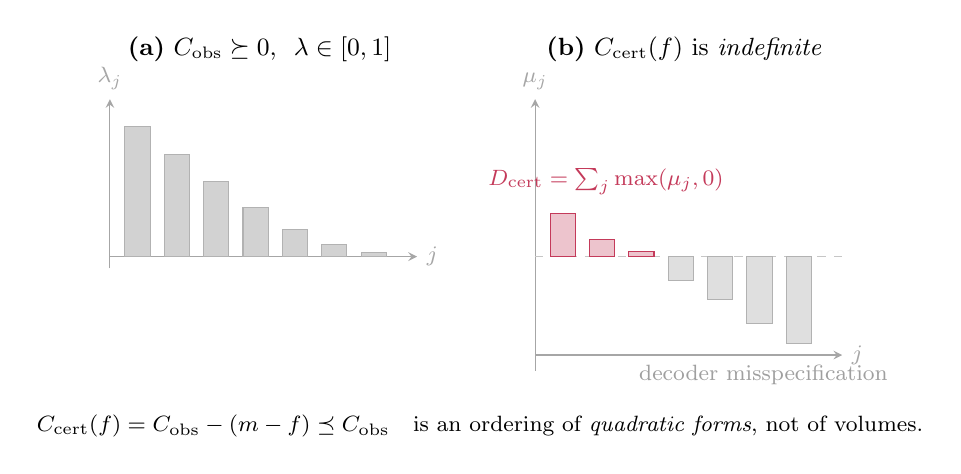
\begin{tikzpicture}[scale=1.0,every node/.style={font=\small}]
  % left: C_obs, PSD, spectrum in [0,1]
  \begin{scope}
    \node[anchor=south,align=center] at (1.9,2.35)
      {\textbf{(a)} $C_{\mathrm{obs}}\succeq 0$, \ $\lambda\in[0,1]$};
    \draw[->,>=stealth,gray!70] (0,0) -- (3.9,0) node[right,font=\footnotesize] {$j$};
    \draw[->,>=stealth,gray!70] (0,-0.15) -- (0,2.0) node[above,font=\footnotesize] {$\lambda_j$};
    \foreach \x/\h in {0.35/1.65,0.85/1.30,1.35/0.95,1.85/0.62,2.35/0.34,2.85/0.15,3.35/0.05}
      \draw[fill=gray!35,draw=gray!60] (\x-0.16,0) rectangle (\x+0.16,\h);
  \end{scope}
  % right: C_cert, indefinite
  \begin{scope}[shift={(5.4,0)}]
    \node[anchor=south,align=center] at (1.9,2.35)
      {\textbf{(b)} $C_{\mathrm{cert}}(f)$ is \emph{indefinite}};
    \draw[->,>=stealth,gray!70] (0,-1.25) -- (3.9,-1.25) node[right,font=\footnotesize] {$j$};
    \draw[->,>=stealth,gray!70] (0,-1.45) -- (0,2.0) node[above,font=\footnotesize] {$\mu_j$};
    \draw[gray!45,dashed] (0,0) -- (3.9,0);
    \foreach \x/\h in {0.35/0.55,0.85/0.22,1.35/0.06}
      \draw[fill=accent!30,draw=accent] (\x-0.16,0) rectangle (\x+0.16,\h);
    \foreach \x/\h in {1.85/-0.30,2.35/-0.55,2.85/-0.85,3.35/-1.10}
      \draw[fill=gray!25,draw=gray!60] (\x-0.16,0) rectangle (\x+0.16,\h);
    \node[font=\footnotesize,accent] at (0.9,0.95) {$D_{\mathrm{cert}}=\sum_j\max(\mu_j,0)$};
    \node[font=\footnotesize,gray!75] at (2.9,-1.5) {decoder misspecification};
  \end{scope}
  \node[font=\footnotesize,align=center] at (4.7,-2.15)
    {$C_{\mathrm{cert}}(f)=C_{\mathrm{obs}}-\Cov(m-f)\preceq C_{\mathrm{obs}}$
     \ \ is an ordering of \emph{quadratic forms}, not of volumes.};
\end{tikzpicture}

\caption{The certificate is not a smaller ellipsoid. (a) $\Cobs$ is positive semidefinite
with eigenvalues in $[0,1]$, so it has an ellipsoid. (b) $\Ccert(f)$ is indefinite: its
positive part is the certified observability mass $\Dcert$, and its negative part measures
where the decoder is misspecified. $\Ccert\preceq\Cobs$ is an ordering of quadratic forms,
so nesting the two as volumes would misstate the object being estimated.}
\label{fig:certificate}
\end{figure}

\paragraph{Estimating it without reading back the decoder's own noise.}
Three separations are required, and each removes a distinct optimism.
\emph{(i) Teacher/operator split.} The decoder is fit on $A_{\mathrm{teacher}}$ and
$\Ccert$ is estimated on a disjoint $A_{\mathrm{operator}}$; sharing them lets the
operator read back the decoder's fitting noise as observability.
\emph{(ii) Held-out spectrum.} Directions are chosen on the fitting split and their
eigenvalues re-estimated on held-out data; in-sample spectra exceed the theoretical bound
of \eqref{eq:quadform} substantially.
\emph{(iii) Inner cross-fit.} Scoring a discovered subspace by
$\Dcert(V)=\sum_j\max(\mu_j,0)$ with $\mu=\mathrm{eig}(V\Ccert^{\mathrm{held}}V^\top)$ is a
max-type functional, so choosing the within-subspace rotation and measuring its eigenvalues
on the same samples rectifies noise into positive mass. The rotation is therefore chosen on
one half of the held-out samples and measured on the other.
The reported quantity is a subspace property: clipping the \emph{diagonal} of
$V\Ccert V^\top$ instead is basis-dependent and can report zero where the subspace contains
a certified direction one rotation away.

\subsection{Receiver-conditional observability}
\label{sec:receiver}

\emph{How does observability depend on what the receiver knows?}

Nothing so far ties $\Cobs$ to $Y$ specifically. Let $\mathcal I_R$ be the receiver's
information set and define $\Cobs(\mathcal I_R)=\Cov(\Exp[Z\mid\mathcal I_R])$. Two
receivers concern us: the blind one, $\mathcal I_b=Y$, and one that additionally knows the
conditioning the generator used, $\mathcal I_s=(Y,S)$. We take $S=C(P)$ to be the
sample-specific conditioning embedding actually supplied to the generator, not the raw
prompt $P$: this asks what happens when the receiver knows what the generator knew, and
keeps the choice of text encoder out of the comparison.

\begin{theorem}[Monotonicity of receiver-conditional observability]
\label{thm:mono}
Let $m_b(Y)=\Exp[Z\mid Y]$ and $m_s(Y,S)=\Exp[Z\mid Y,S]$. Then
\[
  \Cobs(Y,S)-\Cobs(Y)\;=\;\Exp\bigl[\Cov(m_s\mid Y)\bigr]\;\succeq\;0 .
\]
\end{theorem}
\begin{proof}
$\Exp[m_s\mid Y]=m_b$ by the tower property, so the law of total covariance gives
$\Cov(m_s)=\Cov(\Exp[m_s\mid Y])+\Exp[\Cov(m_s\mid Y)]=\Cov(m_b)+\Exp[\Cov(m_s\mid Y)]$.
\end{proof}

\noindent\textbf{Consequence.} Observability is not a property of the channel alone. Side
information can only enlarge the observable geometry, and the gain
$\Delta C_{\mathrm{side}}=\Exp[\Cov(m_s\mid Y)]$ has a direct reading: how much the
posterior mean still moves once $Y$ is known.

\paragraph{The estimator does not inherit the ordering.}
Theorem~\ref{thm:mono} is about Bayes quantities. With two \emph{approximate} decoders,
\begin{equation}
  \Ccert^{\mathrm{side}}(f_s)-\Ccert^{\mathrm{blind}}(f_b)
  \;=\;\Delta C_{\mathrm{side}}-(E_s-E_b),\qquad
  E_s=\Cov(m_s-f_s),\ E_b=\Cov(m_b-f_b),
  \label{eq:contrast}
\end{equation}
so the estimated difference can have negative eigenvalues although the population
difference cannot, and can equally \emph{overstate} the gain when the side decoder fits
more easily ($E_s<E_b$). Neither $E_s$ nor $E_b$ is observable, and no matching of
architecture, budget or training loss identifies them: $\mathrm{MSE}(f)=\mathrm{MMSE}+
\text{approximation error}$, and side information changes the irreducible term itself. We
therefore call \eqref{eq:contrast} the \emph{decoder-certified side-information
contrast}, never a certified gain, and register in advance that a statistically credible
negative direction in it invalidates a Bayes-level reading rather than showing that side
information hurts.

\subsection{From observability geometry to operational coordinates}
\label{sec:operational}

\emph{How do observable directions become operational coordinates?}

Let $V_k=[v_1,\dots,v_k]^\top$ be the leading $k$ rows of the certified spectrum and define
the latent coordinates
\begin{equation}
  W \;=\; V_kZ .
  \label{eq:coords}
\end{equation}
Because $V_kV_k^\top=I_k$ and $Z\sim\mathcal N(0,I)$, we have $W\sim\mathcal N(0,I_k)$
exactly: choosing a subspace changes which coordinates are read, not the prior they are
read against. This is what makes different choices of $V_k$ comparable at all.

Geometry discovery and operational evaluation are then kept apart. $V_k$ is discovered from
$\Ccert$ on the discovery split and frozen; a \emph{fresh} receiver $H(Y)$ --- or
$H(Y,S)$ --- is trained on a disjoint split to predict $W$, and is evaluated on held-out
samples under a fixed set of channel perturbations. We report sign bit error rate, the
linear explained variance $R^2_{\mathrm{lin}}=\frac1k\sum_j\rho_j^2$, and coordinate MSE.

\paragraph{Operational hypothesis, not a theorem.}
The framework predicts an ordering:
\begin{equation}
  \Dcert(V_a)>\Dcert(V_b)\ \Longrightarrow\ V_a\ \text{should show better held-out
  recoverability than}\ V_b .
  \label{eq:hypothesis}
\end{equation}
This is an empirical claim about a trained receiver, not a consequence of
Theorem~\ref{thm:cert}, and we test it rather than assume it. A geometry-free reference is
available throughout: a Haar-random $k$-frame $V_{\mathrm{Haar}}$, which is the correct
null for ``the channel is anisotropic'' because it is a uniformly drawn subspace rather
than a structured one.

\section{Experiments}

\textbf{[Phase A running; this section is written once the four-arm ladder completes. The
subsections below name the questions, in the order they were registered.]}

\subsection{Does the certified estimator recover a known geometry?}
Synthetic linear--Gaussian channels where $\Cobs$ is available in closed form via
Proposition~\ref{prop:fisher}.

\subsection{Is the observability of a real diffusion channel anisotropic?}
Stable Diffusion v1.5, DDIM, frozen; certified spectra and their architecture dependence.

\subsection{Do certified directions predict held-out recoverability?}
A direct test of \eqref{eq:hypothesis} against the Haar null.

\subsection{Does the receiver's information set change what is observable?}
The four-arm ladder: $f(Y)$, $f(Y,S_{\mathrm{null}})$, $f(Y,S_{\mathrm{shuffled}})$,
$f(Y,S_{\mathrm{correct}})$, with the primary contrast isolating \emph{paired}
conditioning from architecture and from the conditioning marginal.

\section{Discussion}

\textbf{[Pending Phase A.]}

\bibliographystyle{iclr2026_conference}
\bibliography{iclr2026_conference}

\end{document}
